% Options for packages loaded elsewhere
\PassOptionsToPackage{unicode}{hyperref}
\PassOptionsToPackage{hyphens}{url}
\PassOptionsToPackage{dvipsnames,svgnames,x11names}{xcolor}
%
\documentclass[
  letterpaper,
  DIV=11,
  numbers=noendperiod]{scrreprt}

\usepackage{amsmath,amssymb}
\usepackage{lmodern}
\usepackage{iftex}
\ifPDFTeX
  \usepackage[T1]{fontenc}
  \usepackage[utf8]{inputenc}
  \usepackage{textcomp} % provide euro and other symbols
\else % if luatex or xetex
  \usepackage{unicode-math}
  \defaultfontfeatures{Scale=MatchLowercase}
  \defaultfontfeatures[\rmfamily]{Ligatures=TeX,Scale=1}
\fi
% Use upquote if available, for straight quotes in verbatim environments
\IfFileExists{upquote.sty}{\usepackage{upquote}}{}
\IfFileExists{microtype.sty}{% use microtype if available
  \usepackage[]{microtype}
  \UseMicrotypeSet[protrusion]{basicmath} % disable protrusion for tt fonts
}{}
\makeatletter
\@ifundefined{KOMAClassName}{% if non-KOMA class
  \IfFileExists{parskip.sty}{%
    \usepackage{parskip}
  }{% else
    \setlength{\parindent}{0pt}
    \setlength{\parskip}{6pt plus 2pt minus 1pt}}
}{% if KOMA class
  \KOMAoptions{parskip=half}}
\makeatother
\usepackage{xcolor}
\setlength{\emergencystretch}{3em} % prevent overfull lines
\setcounter{secnumdepth}{5}
% Make \paragraph and \subparagraph free-standing
\ifx\paragraph\undefined\else
  \let\oldparagraph\paragraph
  \renewcommand{\paragraph}[1]{\oldparagraph{#1}\mbox{}}
\fi
\ifx\subparagraph\undefined\else
  \let\oldsubparagraph\subparagraph
  \renewcommand{\subparagraph}[1]{\oldsubparagraph{#1}\mbox{}}
\fi

\usepackage{color}
\usepackage{fancyvrb}
\newcommand{\VerbBar}{|}
\newcommand{\VERB}{\Verb[commandchars=\\\{\}]}
\DefineVerbatimEnvironment{Highlighting}{Verbatim}{commandchars=\\\{\}}
% Add ',fontsize=\small' for more characters per line
\usepackage{framed}
\definecolor{shadecolor}{RGB}{241,243,245}
\newenvironment{Shaded}{\begin{snugshade}}{\end{snugshade}}
\newcommand{\AlertTok}[1]{\textcolor[rgb]{0.68,0.00,0.00}{#1}}
\newcommand{\AnnotationTok}[1]{\textcolor[rgb]{0.37,0.37,0.37}{#1}}
\newcommand{\AttributeTok}[1]{\textcolor[rgb]{0.40,0.45,0.13}{#1}}
\newcommand{\BaseNTok}[1]{\textcolor[rgb]{0.68,0.00,0.00}{#1}}
\newcommand{\BuiltInTok}[1]{\textcolor[rgb]{0.00,0.23,0.31}{#1}}
\newcommand{\CharTok}[1]{\textcolor[rgb]{0.13,0.47,0.30}{#1}}
\newcommand{\CommentTok}[1]{\textcolor[rgb]{0.37,0.37,0.37}{#1}}
\newcommand{\CommentVarTok}[1]{\textcolor[rgb]{0.37,0.37,0.37}{\textit{#1}}}
\newcommand{\ConstantTok}[1]{\textcolor[rgb]{0.56,0.35,0.01}{#1}}
\newcommand{\ControlFlowTok}[1]{\textcolor[rgb]{0.00,0.23,0.31}{#1}}
\newcommand{\DataTypeTok}[1]{\textcolor[rgb]{0.68,0.00,0.00}{#1}}
\newcommand{\DecValTok}[1]{\textcolor[rgb]{0.68,0.00,0.00}{#1}}
\newcommand{\DocumentationTok}[1]{\textcolor[rgb]{0.37,0.37,0.37}{\textit{#1}}}
\newcommand{\ErrorTok}[1]{\textcolor[rgb]{0.68,0.00,0.00}{#1}}
\newcommand{\ExtensionTok}[1]{\textcolor[rgb]{0.00,0.23,0.31}{#1}}
\newcommand{\FloatTok}[1]{\textcolor[rgb]{0.68,0.00,0.00}{#1}}
\newcommand{\FunctionTok}[1]{\textcolor[rgb]{0.28,0.35,0.67}{#1}}
\newcommand{\ImportTok}[1]{\textcolor[rgb]{0.00,0.46,0.62}{#1}}
\newcommand{\InformationTok}[1]{\textcolor[rgb]{0.37,0.37,0.37}{#1}}
\newcommand{\KeywordTok}[1]{\textcolor[rgb]{0.00,0.23,0.31}{#1}}
\newcommand{\NormalTok}[1]{\textcolor[rgb]{0.00,0.23,0.31}{#1}}
\newcommand{\OperatorTok}[1]{\textcolor[rgb]{0.37,0.37,0.37}{#1}}
\newcommand{\OtherTok}[1]{\textcolor[rgb]{0.00,0.23,0.31}{#1}}
\newcommand{\PreprocessorTok}[1]{\textcolor[rgb]{0.68,0.00,0.00}{#1}}
\newcommand{\RegionMarkerTok}[1]{\textcolor[rgb]{0.00,0.23,0.31}{#1}}
\newcommand{\SpecialCharTok}[1]{\textcolor[rgb]{0.37,0.37,0.37}{#1}}
\newcommand{\SpecialStringTok}[1]{\textcolor[rgb]{0.13,0.47,0.30}{#1}}
\newcommand{\StringTok}[1]{\textcolor[rgb]{0.13,0.47,0.30}{#1}}
\newcommand{\VariableTok}[1]{\textcolor[rgb]{0.07,0.07,0.07}{#1}}
\newcommand{\VerbatimStringTok}[1]{\textcolor[rgb]{0.13,0.47,0.30}{#1}}
\newcommand{\WarningTok}[1]{\textcolor[rgb]{0.37,0.37,0.37}{\textit{#1}}}

\providecommand{\tightlist}{%
  \setlength{\itemsep}{0pt}\setlength{\parskip}{0pt}}\usepackage{longtable,booktabs,array}
\usepackage{calc} % for calculating minipage widths
% Correct order of tables after \paragraph or \subparagraph
\usepackage{etoolbox}
\makeatletter
\patchcmd\longtable{\par}{\if@noskipsec\mbox{}\fi\par}{}{}
\makeatother
% Allow footnotes in longtable head/foot
\IfFileExists{footnotehyper.sty}{\usepackage{footnotehyper}}{\usepackage{footnote}}
\makesavenoteenv{longtable}
\usepackage{graphicx}
\makeatletter
\def\maxwidth{\ifdim\Gin@nat@width>\linewidth\linewidth\else\Gin@nat@width\fi}
\def\maxheight{\ifdim\Gin@nat@height>\textheight\textheight\else\Gin@nat@height\fi}
\makeatother
% Scale images if necessary, so that they will not overflow the page
% margins by default, and it is still possible to overwrite the defaults
% using explicit options in \includegraphics[width, height, ...]{}
\setkeys{Gin}{width=\maxwidth,height=\maxheight,keepaspectratio}
% Set default figure placement to htbp
\makeatletter
\def\fps@figure{htbp}
\makeatother
\newlength{\cslhangindent}
\setlength{\cslhangindent}{1.5em}
\newlength{\csllabelwidth}
\setlength{\csllabelwidth}{3em}
\newlength{\cslentryspacingunit} % times entry-spacing
\setlength{\cslentryspacingunit}{\parskip}
\newenvironment{CSLReferences}[2] % #1 hanging-ident, #2 entry spacing
 {% don't indent paragraphs
  \setlength{\parindent}{0pt}
  % turn on hanging indent if param 1 is 1
  \ifodd #1
  \let\oldpar\par
  \def\par{\hangindent=\cslhangindent\oldpar}
  \fi
  % set entry spacing
  \setlength{\parskip}{#2\cslentryspacingunit}
 }%
 {}
\usepackage{calc}
\newcommand{\CSLBlock}[1]{#1\hfill\break}
\newcommand{\CSLLeftMargin}[1]{\parbox[t]{\csllabelwidth}{#1}}
\newcommand{\CSLRightInline}[1]{\parbox[t]{\linewidth - \csllabelwidth}{#1}\break}
\newcommand{\CSLIndent}[1]{\hspace{\cslhangindent}#1}

<script src="site_libs/htmlwidgets-1.6.0/htmlwidgets.js"></script>
<script src="site_libs/jquery-3.6.0/jquery-3.6.0.min.js"></script>
<link href="site_libs/leaflet-1.3.1/leaflet.css" rel="stylesheet" />
<script src="site_libs/leaflet-1.3.1/leaflet.js"></script>
<link href="site_libs/leafletfix-1.0.0/leafletfix.css" rel="stylesheet" />
<script src="site_libs/proj4-2.6.2/proj4.min.js"></script>
<script src="site_libs/Proj4Leaflet-1.0.1/proj4leaflet.js"></script>
<link href="site_libs/rstudio_leaflet-1.3.1/rstudio_leaflet.css" rel="stylesheet" />
<script src="site_libs/leaflet-binding-2.1.1.9000/leaflet.js"></script>
<script src="site_libs/plotly-binding-4.10.1/plotly.js"></script>
<script src="site_libs/setprototypeof-0.1/setprototypeof.js"></script>
<script src="site_libs/typedarray-0.1/typedarray.min.js"></script>
<link href="site_libs/crosstalk-1.2.0/css/crosstalk.min.css" rel="stylesheet" />
<script src="site_libs/crosstalk-1.2.0/js/crosstalk.min.js"></script>
<link href="site_libs/plotly-htmlwidgets-css-2.11.1/plotly-htmlwidgets.css" rel="stylesheet" />
<script src="site_libs/plotly-main-2.11.1/plotly-latest.min.js"></script>
<script src="site_libs/ionrangeslider-javascript-2.3.1/js/ion.rangeSlider.min.js"></script>
<script src="site_libs/strftime-0.9.2/strftime-min.js"></script>
<link href="site_libs/ionrangeslider-css-2.3.1/css/ion.rangeSlider.css" rel="stylesheet" />
<link href="site_libs/leaflet-easybutton-1.3.1/easy-button.css" rel="stylesheet" />
<script src="site_libs/leaflet-easybutton-1.3.1/easy-button.js"></script>
<script src="site_libs/leaflet-easybutton-1.3.1/EasyButton-binding.js"></script>
<link href="site_libs/leaflet-locationfilter2-0.1.1/locationfilter.css" rel="stylesheet" />
<script src="site_libs/leaflet-locationfilter2-0.1.1/locationfilter.js"></script>
<script src="site_libs/leaflet-locationfilter2-0.1.1/locationfilter-bindings.js"></script>
<link href="site_libs/ionicons-2.0.1/ionicons.min.css" rel="stylesheet" />
<link href="site_libs/datatables-css-0.0.0/datatables-crosstalk.css" rel="stylesheet" />
<script src="site_libs/datatables-binding-0.26/datatables.js"></script>
<link href="site_libs/dt-core-bootstrap-1.12.1/css/dataTables.bootstrap.min.css" rel="stylesheet" />
<link href="site_libs/dt-core-bootstrap-1.12.1/css/dataTables.bootstrap.extra.css" rel="stylesheet" />
<script src="site_libs/dt-core-bootstrap-1.12.1/js/jquery.dataTables.min.js"></script>
<script src="site_libs/dt-core-bootstrap-1.12.1/js/dataTables.bootstrap.min.js"></script>
<link href="site_libs/dt-ext-scroller-bootstrap-1.12.1/css/scroller.bootstrap.min.css" rel="stylesheet" />
<script src="site_libs/dt-ext-scroller-bootstrap-1.12.1/js/dataTables.scroller.min.js"></script>
<script src="site_libs/dt-ext-scroller-bootstrap-1.12.1/js/scroller.bootstrap.min.js"></script>
<meta name="viewport" content="width=device-width, initial-scale=1" />
<link href="site_libs/bootstrap-grid-3.4.1/bootstrap-grid.min.css" rel="stylesheet" />
\KOMAoption{captions}{tableheading}
\makeatletter
\makeatother
\makeatletter
\@ifpackageloaded{bookmark}{}{\usepackage{bookmark}}
\makeatother
\makeatletter
\@ifpackageloaded{caption}{}{\usepackage{caption}}
\AtBeginDocument{%
\ifdefined\contentsname
  \renewcommand*\contentsname{Table of contents}
\else
  \newcommand\contentsname{Table of contents}
\fi
\ifdefined\listfigurename
  \renewcommand*\listfigurename{List of Figures}
\else
  \newcommand\listfigurename{List of Figures}
\fi
\ifdefined\listtablename
  \renewcommand*\listtablename{List of Tables}
\else
  \newcommand\listtablename{List of Tables}
\fi
\ifdefined\figurename
  \renewcommand*\figurename{Figure}
\else
  \newcommand\figurename{Figure}
\fi
\ifdefined\tablename
  \renewcommand*\tablename{Table}
\else
  \newcommand\tablename{Table}
\fi
}
\@ifpackageloaded{float}{}{\usepackage{float}}
\floatstyle{ruled}
\@ifundefined{c@chapter}{\newfloat{codelisting}{h}{lop}}{\newfloat{codelisting}{h}{lop}[chapter]}
\floatname{codelisting}{Listing}
\newcommand*\listoflistings{\listof{codelisting}{List of Listings}}
\makeatother
\makeatletter
\@ifpackageloaded{caption}{}{\usepackage{caption}}
\@ifpackageloaded{subcaption}{}{\usepackage{subcaption}}
\makeatother
\makeatletter
\@ifpackageloaded{tcolorbox}{}{\usepackage[many]{tcolorbox}}
\makeatother
\makeatletter
\@ifundefined{shadecolor}{\definecolor{shadecolor}{rgb}{.97, .97, .97}}
\makeatother
\makeatletter
\makeatother
\ifLuaTeX
  \usepackage{selnolig}  % disable illegal ligatures
\fi
\IfFileExists{bookmark.sty}{\usepackage{bookmark}}{\usepackage{hyperref}}
\IfFileExists{xurl.sty}{\usepackage{xurl}}{} % add URL line breaks if available
\urlstyle{same} % disable monospaced font for URLs
\hypersetup{
  pdftitle={shiny-workshop},
  pdfauthor={Jane Doe},
  colorlinks=true,
  linkcolor={blue},
  filecolor={Maroon},
  citecolor={Blue},
  urlcolor={Blue},
  pdfcreator={LaTeX via pandoc}}

\title{shiny-workshop}
\author{Jane Doe}
\date{3/6/23}

\begin{document}
\maketitle
\ifdefined\Shaded\renewenvironment{Shaded}{\begin{tcolorbox}[frame hidden, sharp corners, boxrule=0pt, borderline west={3pt}{0pt}{shadecolor}, breakable, interior hidden, enhanced]}{\end{tcolorbox}}\fi

\renewcommand*\contentsname{Table of contents}
{
\hypersetup{linkcolor=}
\setcounter{tocdepth}{2}
\tableofcontents
}
\bookmarksetup{startatroot}

\hypertarget{preface}{%
\chapter*{Preface}\label{preface}}
\addcontentsline{toc}{chapter}{Preface}

\markboth{Preface}{Preface}

This is a Quarto book.

To learn more about Quarto books visit
\url{https://quarto.org/docs/books}.

\begin{Shaded}
\begin{Highlighting}[]
\DecValTok{1} \SpecialCharTok{+} \DecValTok{1}
\end{Highlighting}
\end{Shaded}

\begin{verbatim}
[1] 2
\end{verbatim}

\bookmarksetup{startatroot}

\hypertarget{introduction}{%
\chapter{Introduction}\label{introduction}}

This is a book created from markdown and executable code.

See Knuth (1984) for additional discussion of literate programming.

\begin{Shaded}
\begin{Highlighting}[]
\DecValTok{1} \SpecialCharTok{+} \DecValTok{1}
\end{Highlighting}
\end{Shaded}

\begin{verbatim}
[1] 2
\end{verbatim}

\bookmarksetup{startatroot}

\hypertarget{shiny-applications}{%
\chapter{Shiny Applications}\label{shiny-applications}}

\hypertarget{learning-objectives}{%
\section*{Learning Objectives}\label{learning-objectives}}
\addcontentsline{toc}{section}{Learning Objectives}

\markright{Learning Objectives}

Use the Shiny framework to develop online interactive applications
accepting user input to render outputs from arbitrary R functions.
Server requirements differentiating from simpler Rmarkdown renderings
will be reviewed as well as use of Crosstalk to gain similar
functionality with Rmarkdown with simple data.

\hypertarget{install-shiny-r-package}{%
\section{\texorpdfstring{Install \texttt{shiny} R
package}{Install shiny R package}}\label{install-shiny-r-package}}

Ensure you have the \texttt{shiny} R package installed. Look in
RStudio's Packages pane and Install if not found when searching for
``shiny''.

A few other packages will get used so let's use the librarian::shelf()
command to install if needed:

\begin{Shaded}
\begin{Highlighting}[]
\NormalTok{librarian}\SpecialCharTok{::}\FunctionTok{shelf}\NormalTok{(}
\NormalTok{  plotly, reactlog, shiny, shinydashboard)}
\end{Highlighting}
\end{Shaded}

\hypertarget{create-your-first-shiny-web-app}{%
\section{Create your first Shiny web
app}\label{create-your-first-shiny-web-app}}

Similar to other examples, let's create a simple Shiny app starting from
the provided default by going to \textbf{File} -\textgreater{}
\textbf{New File} -\textgreater{} \textbf{Shiny Web App}\ldots{} and
name it \textbf{\emph{app-faithful}} (after
\href{https://www.rdocumentation.org/packages/datasets/versions/3.6.2/topics/faithful}{faithful},
the Old Faithful geyser eruption frequency dataset used in this default
example):

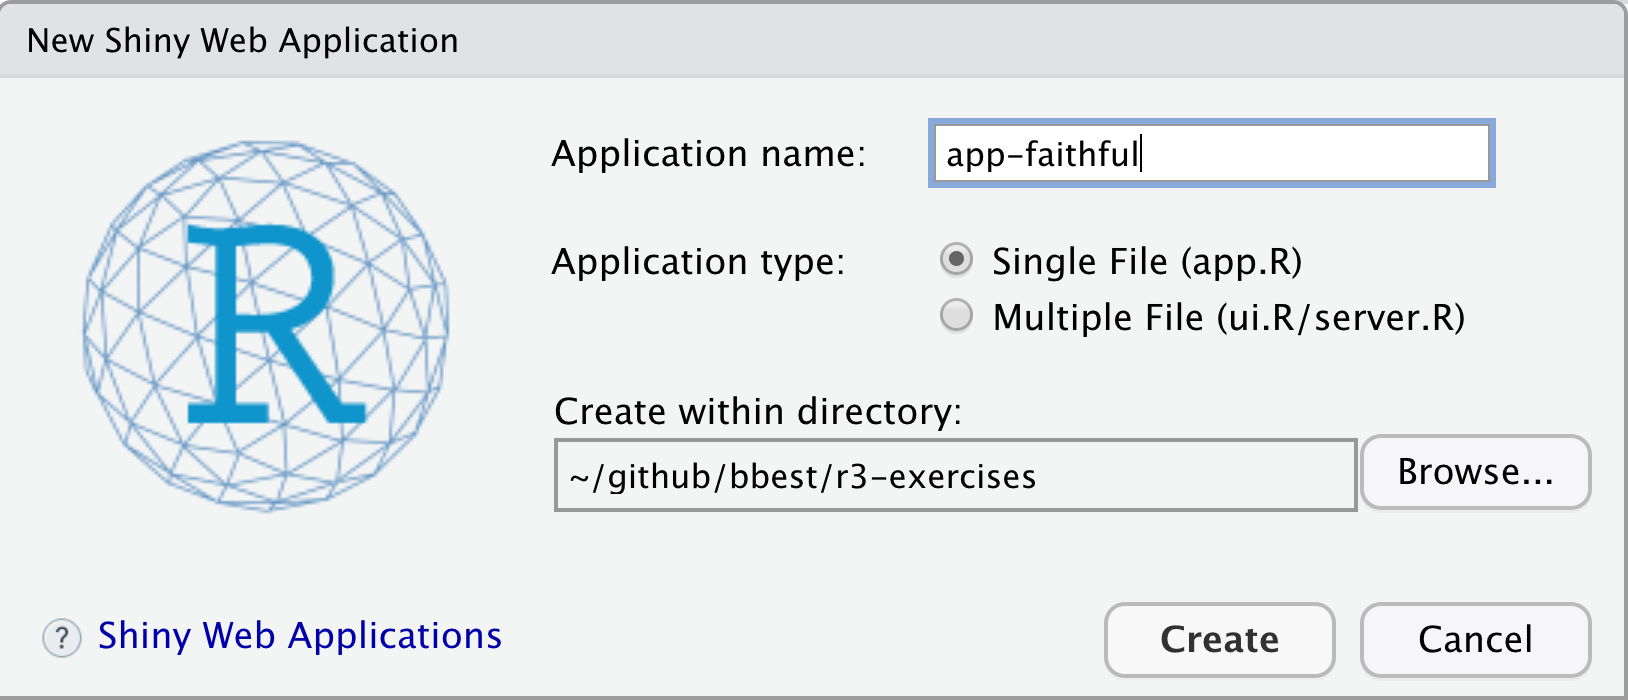
\includegraphics[width=4.16667in,height=\textheight]{./figs/shiny/new-shiny_app-faithful.png}

For now, let's go with the default \textbf{Single File} option that puts
the entire application in \texttt{app.R} rather than splitting it in two
(\texttt{ui.R}/\texttt{server.R}). You should see the following contents
in the new \texttt{app.R} file contents:

\begin{Shaded}
\begin{Highlighting}[]
\CommentTok{\#}
\CommentTok{\# This is a Shiny web application. You can run the application by clicking}
\CommentTok{\# the \textquotesingle{}Run App\textquotesingle{} button above.}
\CommentTok{\#}
\CommentTok{\# Find out more about building applications with Shiny here:}
\CommentTok{\#}
\CommentTok{\#    http://shiny.rstudio.com/}
\CommentTok{\#}

\FunctionTok{library}\NormalTok{(shiny)}

\CommentTok{\# Define UI for application that draws a histogram}
\NormalTok{ui }\OtherTok{\textless{}{-}} \FunctionTok{fluidPage}\NormalTok{(}

    \CommentTok{\# Application title}
    \FunctionTok{titlePanel}\NormalTok{(}\StringTok{"Old Faithful Geyser Data"}\NormalTok{),}

    \CommentTok{\# Sidebar with a slider input for number of bins }
    \FunctionTok{sidebarLayout}\NormalTok{(}
        \FunctionTok{sidebarPanel}\NormalTok{(}
            \FunctionTok{sliderInput}\NormalTok{(}\StringTok{"bins"}\NormalTok{,}
                        \StringTok{"Number of bins:"}\NormalTok{,}
                        \AttributeTok{min =} \DecValTok{1}\NormalTok{,}
                        \AttributeTok{max =} \DecValTok{50}\NormalTok{,}
                        \AttributeTok{value =} \DecValTok{30}\NormalTok{)}
\NormalTok{        ),}

        \CommentTok{\# Show a plot of the generated distribution}
        \FunctionTok{mainPanel}\NormalTok{(}
           \FunctionTok{plotOutput}\NormalTok{(}\StringTok{"distPlot"}\NormalTok{)}
\NormalTok{        )}
\NormalTok{    )}
\NormalTok{)}

\CommentTok{\# Define server logic required to draw a histogram}
\NormalTok{server }\OtherTok{\textless{}{-}} \ControlFlowTok{function}\NormalTok{(input, output) \{}

\NormalTok{    output}\SpecialCharTok{$}\NormalTok{distPlot }\OtherTok{\textless{}{-}} \FunctionTok{renderPlot}\NormalTok{(\{}
        \CommentTok{\# generate bins based on input$bins from ui.R}
\NormalTok{        x    }\OtherTok{\textless{}{-}}\NormalTok{ faithful[, }\DecValTok{2}\NormalTok{]}
\NormalTok{        bins }\OtherTok{\textless{}{-}} \FunctionTok{seq}\NormalTok{(}\FunctionTok{min}\NormalTok{(x), }\FunctionTok{max}\NormalTok{(x), }\AttributeTok{length.out =}\NormalTok{ input}\SpecialCharTok{$}\NormalTok{bins }\SpecialCharTok{+} \DecValTok{1}\NormalTok{)}

        \CommentTok{\# draw the histogram with the specified number of bins}
        \FunctionTok{hist}\NormalTok{(x, }\AttributeTok{breaks =}\NormalTok{ bins, }\AttributeTok{col =} \StringTok{\textquotesingle{}darkgray\textquotesingle{}}\NormalTok{, }\AttributeTok{border =} \StringTok{\textquotesingle{}white\textquotesingle{}}\NormalTok{)}
\NormalTok{    \})}
\NormalTok{\}}

\CommentTok{\# Run the application }
\FunctionTok{shinyApp}\NormalTok{(}\AttributeTok{ui =}\NormalTok{ ui, }\AttributeTok{server =}\NormalTok{ server)}
\end{Highlighting}
\end{Shaded}

Let's next \textbf{Run App}. Note that you can change the options by
clicking on the down triangle next to the button, such as running the
app in your default web browser (\textbf{\emph{Run External}}), a pop-up
window or in RStudio's Viewer Pane.

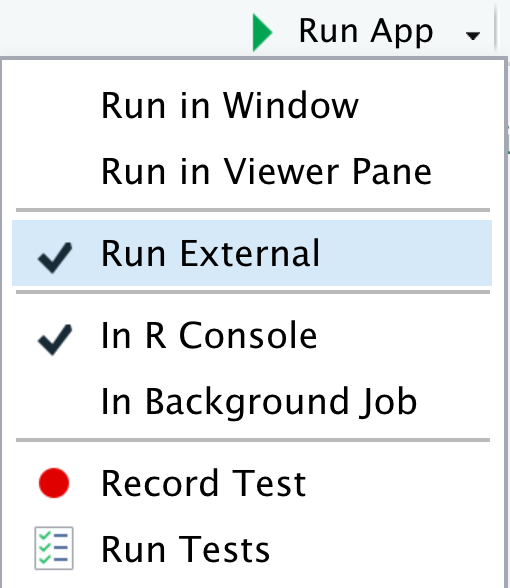
\includegraphics[width=2.08333in,height=\textheight]{./figs/shiny/shiny-run-app-options.png}

Now you can change the values in the slider on the left, then see the
plot updated:

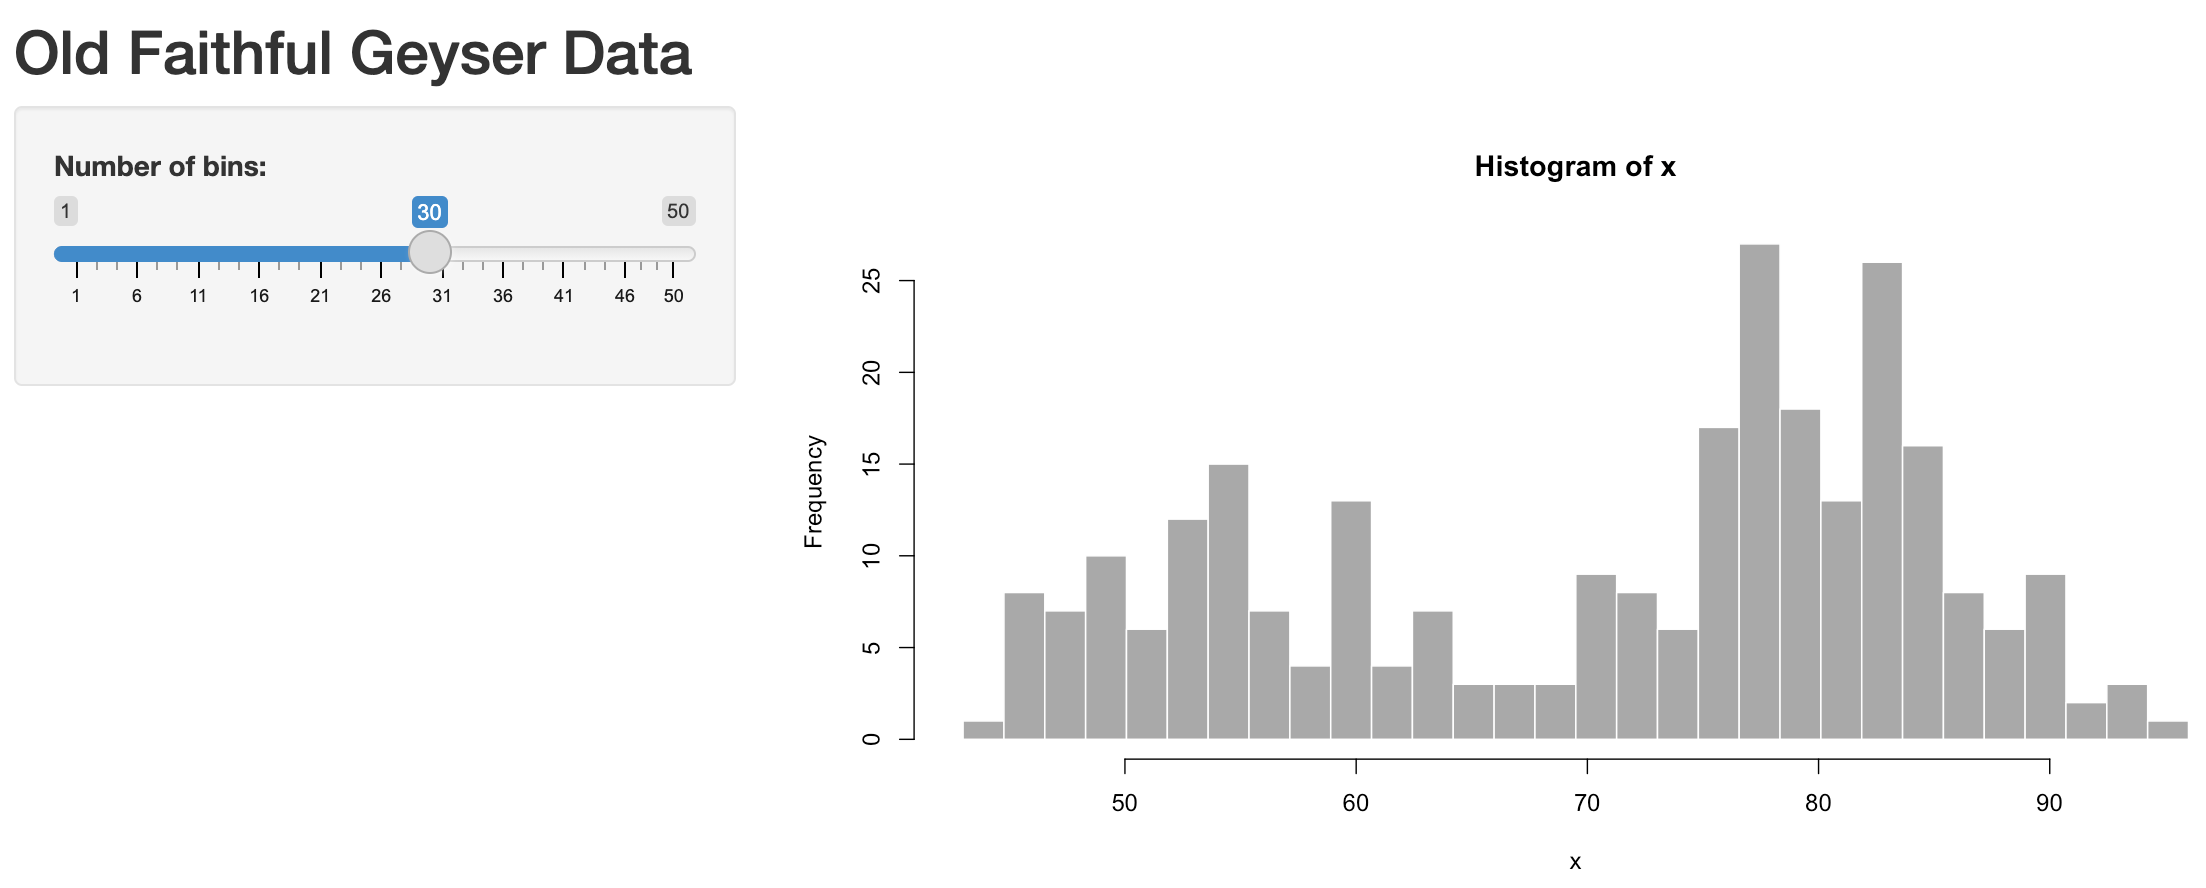
\includegraphics[width=6.25in,height=\textheight]{./figs/shiny/faithful-app.png}

In Shiny parlance, the histogram plot is \textbf{\emph{reactive}} to the
slider. Normally when creating web apps, this type of ``reactivity'' is
quite complicated to code, but here by simply using \texttt{input\$bins}
in the plotting function for the \texttt{output\$distPlot}, Shiny
registers that this plot needs to be updated when the user changes the
\texttt{input\$bins} value.

\hypertarget{run-in-showcase-mode}{%
\subsection{Run in showcase mode}\label{run-in-showcase-mode}}

This default example along with other are made available in the shiny
package's installed folder:

\begin{Shaded}
\begin{Highlighting}[]
\CommentTok{\# get path to "examples" under your installation of the Shiny R package}
\NormalTok{dir\_examples  }\OtherTok{\textless{}{-}} \FunctionTok{system.file}\NormalTok{(}\StringTok{"examples"}\NormalTok{, }\AttributeTok{package=}\StringTok{"shiny"}\NormalTok{)}

\CommentTok{\# get all directories listed there}
\NormalTok{dirs\_examples }\OtherTok{\textless{}{-}} \FunctionTok{list.dirs}\NormalTok{(dir\_examples, }\AttributeTok{recursive =}\NormalTok{ F)}

\CommentTok{\# show the folder name only, not the rest of the path preceding (ie dirname())}
\FunctionTok{basename}\NormalTok{(dirs\_examples)}
\end{Highlighting}
\end{Shaded}

\begin{verbatim}
 [1] "01_hello"      "02_text"       "03_reactivity" "04_mpg"       
 [5] "05_sliders"    "06_tabsets"    "07_widgets"    "08_html"      
 [9] "09_upload"     "10_download"   "11_timer"     
\end{verbatim}

Another way to launch the shiny app is with the following:

\begin{Shaded}
\begin{Highlighting}[]
\CommentTok{\# set directory to 01\_hello app, aka the simplest default faithful app}
\NormalTok{dir\_hello\_app }\OtherTok{\textless{}{-}} \FunctionTok{file.path}\NormalTok{(dir\_examples, }\StringTok{"01\_hello"}\NormalTok{)}

\CommentTok{\# run the app with display.mode = "auto"}
\CommentTok{\#   which under shiny R package uses "showcase" mode because of the DESCRIPTION  file there (see ?shiny::runApp)}
\NormalTok{shiny}\SpecialCharTok{::}\FunctionTok{runApp}\NormalTok{(dir\_hello\_app)}
\end{Highlighting}
\end{Shaded}

\hypertarget{download-run-examples}{%
\section{Download \& run examples}\label{download-run-examples}}

Next, let's go through examples together.

Download
\href{https://github.com/bbest/shiny-intro/archive/master.zip}{shiny-intro-master.zip}
into your \texttt{r3-exercises/}, unzip it and rename the top-level
folder to \texttt{apps/} so you can see the following application
folders directly under \texttt{r3-exercises/apps/}:

\begin{itemize}
\tightlist
\item
  \texttt{01\_faithful}: default app from using RStudio, File
  \textgreater{} New File \textgreater{} Shiny Web App\ldots{}
  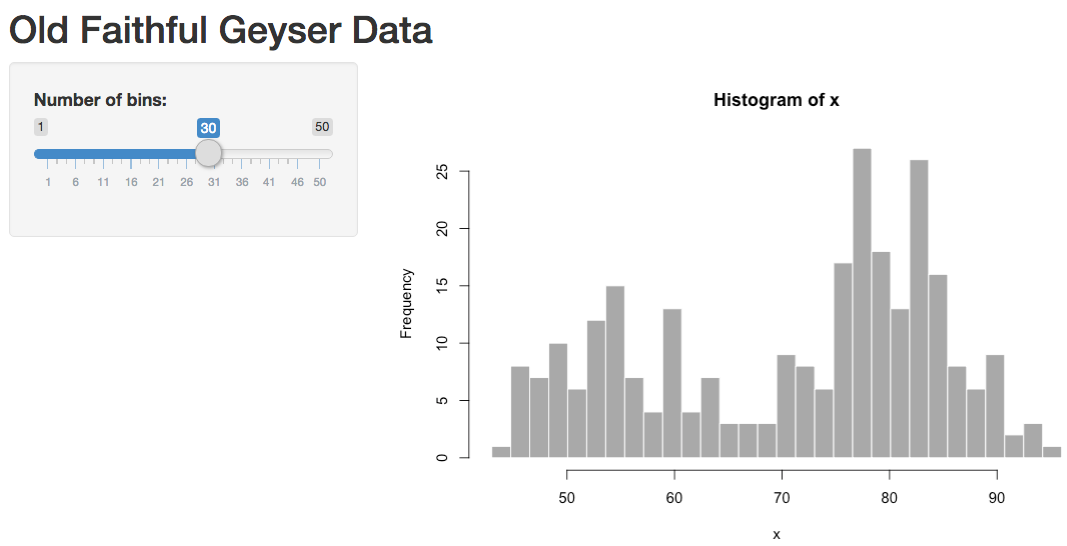
\includegraphics{./figs/shiny/screenshot-01_faithful.png}
\item
  \texttt{02\_quakes\_mag}: swap to quakes dataset, adjust histogram by
  magnitude
\item
  \texttt{03\_quakes\_depth}: add depth slider, select box for variable
  to histogram
\item
  \texttt{04\_quakes\_map}: add leaflet map
\item
  \texttt{05\_quakes\_dashboard}: enhance user interface (ie ``ui'')
  with \texttt{shinydashboard}
  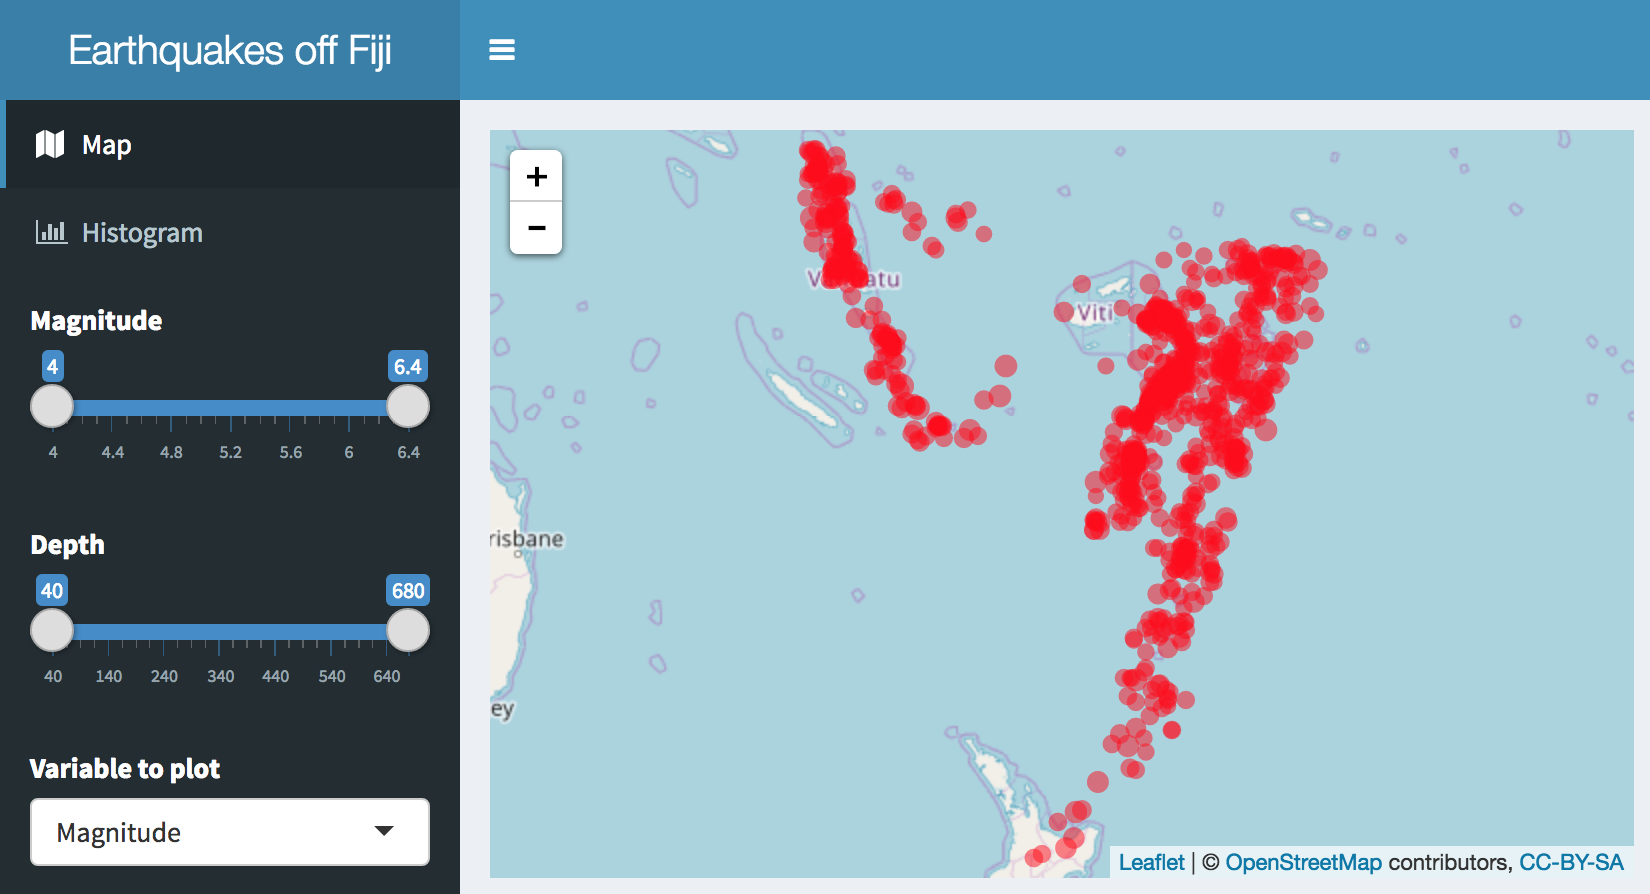
\includegraphics{./figs/shiny/screenshot-05_quakes_dashboard.png}
\end{itemize}

Numbered folders in this repository correspond with iterative
development and enhancement of a Shiny app.

The following sections in this Rmarkdown document demonstrate how you
can develop output visualizations for use in a Shiny app, especially by
defining input variables as a list (\texttt{input\$*}).

Knitting Rmarkdown documents and pushing to Github then allows the HTML
to be viewable (using the \href{https://pages.github.com}{Github Pages}
feature). In contrast, Github and most web hosting services can
\textbf{\emph{not}} host a Shiny app. Although the
\href{http://rstudio.github.io/leaflet}{leaflet} and
\href{https://plot.ly/ggplot2}{plotly} visualizations in this document
are interactive in the web browser, they do not require the Shiny
library or a Shiny server to be displayed. Rather, the HTML output can
be easily hosted on the most basic web server or passed as an email
attachment. The Shiny context allows for ultimate flexibility with user
interactions, but may be overkill for basic visualization. Check out all
the amazing \href{http://www.htmlwidgets.org/}{htmlwidgets.org} and
framework that works in the three contexts of: 1) RStudio, 2) Rmarkdown,
and 3) Shiny.

\hypertarget{faithful}{%
\subsection{\texorpdfstring{\texttt{01\_faithful}}{01\_faithful}}\label{faithful}}

\begin{itemize}
\item
  Code:
  \href{https://github.com/bbest/shiny-intro/tree/master/01_faithful}{01\_faithful}
\item
  Run from GitHub:

\begin{Shaded}
\begin{Highlighting}[]
\NormalTok{shiny}\SpecialCharTok{::}\FunctionTok{runGitHub}\NormalTok{(}\StringTok{"bbest/shiny{-}intro"}\NormalTok{, }\AttributeTok{subdir=}\StringTok{"01\_faithful"}\NormalTok{)}
\end{Highlighting}
\end{Shaded}
\item
  Run locally:

\begin{Shaded}
\begin{Highlighting}[]
\NormalTok{shiny}\SpecialCharTok{::}\FunctionTok{runApp}\NormalTok{(}\StringTok{"01\_faithful"}\NormalTok{)}
\end{Highlighting}
\end{Shaded}
\end{itemize}

In order to quickly experiment with visualization, we could pull the
code from within the rendering function of the Shiny app and set the
input list values that would otherwise be set from the user
interface\ldots{}

\begin{Shaded}
\begin{Highlighting}[]
\NormalTok{input }\OtherTok{=} \FunctionTok{list}\NormalTok{(}\AttributeTok{bins =} \DecValTok{30}\NormalTok{)}

\NormalTok{x }\OtherTok{\textless{}{-}}\NormalTok{ faithful[, }\DecValTok{2}\NormalTok{] }
\NormalTok{bins }\OtherTok{\textless{}{-}} \FunctionTok{seq}\NormalTok{(}\FunctionTok{min}\NormalTok{(x), }\FunctionTok{max}\NormalTok{(x), }\AttributeTok{length.out =}\NormalTok{ input}\SpecialCharTok{$}\NormalTok{bins }\SpecialCharTok{+} \DecValTok{1}\NormalTok{)}
    
\FunctionTok{hist}\NormalTok{(x, }\AttributeTok{breaks =}\NormalTok{ bins, }\AttributeTok{col =} \StringTok{\textquotesingle{}darkgray\textquotesingle{}}\NormalTok{, }\AttributeTok{border =} \StringTok{\textquotesingle{}white\textquotesingle{}}\NormalTok{)}
\end{Highlighting}
\end{Shaded}

\begin{figure}[H]

{\centering 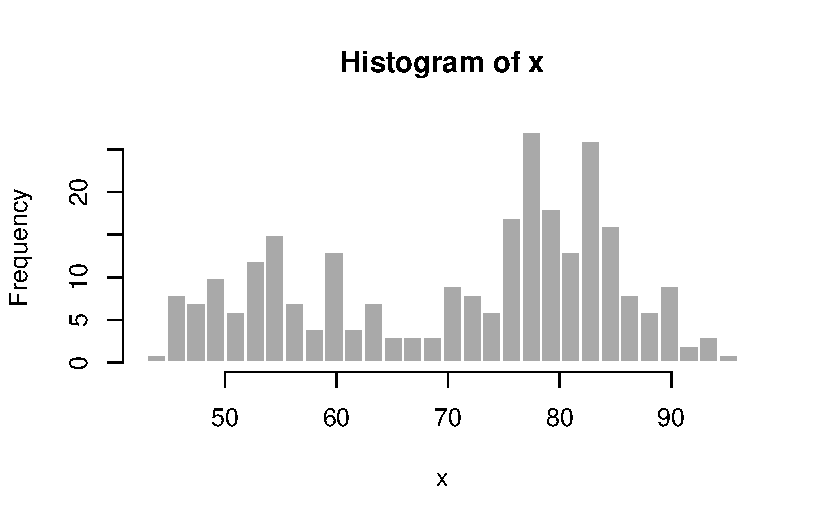
\includegraphics{./shiny_files/figure-pdf/unnamed-chunk-5-1.pdf}

}

\end{figure}

\hypertarget{quakes_mag}{%
\subsection{\texorpdfstring{\texttt{02\_quakes\_mag}}{02\_quakes\_mag}}\label{quakes_mag}}

\begin{Shaded}
\begin{Highlighting}[]
\FunctionTok{library}\NormalTok{(tidyverse)}

\NormalTok{input }\OtherTok{\textless{}{-}} \FunctionTok{list}\NormalTok{(}\AttributeTok{slider\_mag =} \FunctionTok{c}\NormalTok{(}\DecValTok{4}\NormalTok{, }\DecValTok{6}\NormalTok{))}

\NormalTok{d }\OtherTok{\textless{}{-}}\NormalTok{ quakes }\SpecialCharTok{\%\textgreater{}\%}
  \FunctionTok{filter}\NormalTok{(}
\NormalTok{    mag }\SpecialCharTok{\textgreater{}=}\NormalTok{ input}\SpecialCharTok{$}\NormalTok{slider\_mag[}\DecValTok{1}\NormalTok{],}
\NormalTok{    mag }\SpecialCharTok{\textless{}=}\NormalTok{ input}\SpecialCharTok{$}\NormalTok{slider\_mag[}\DecValTok{2}\NormalTok{])}

\FunctionTok{hist}\NormalTok{(d}\SpecialCharTok{$}\NormalTok{mag, }\AttributeTok{col =} \StringTok{\textquotesingle{}darkgray\textquotesingle{}}\NormalTok{, }\AttributeTok{border =} \StringTok{\textquotesingle{}white\textquotesingle{}}\NormalTok{)}
\end{Highlighting}
\end{Shaded}

\begin{figure}[H]

{\centering 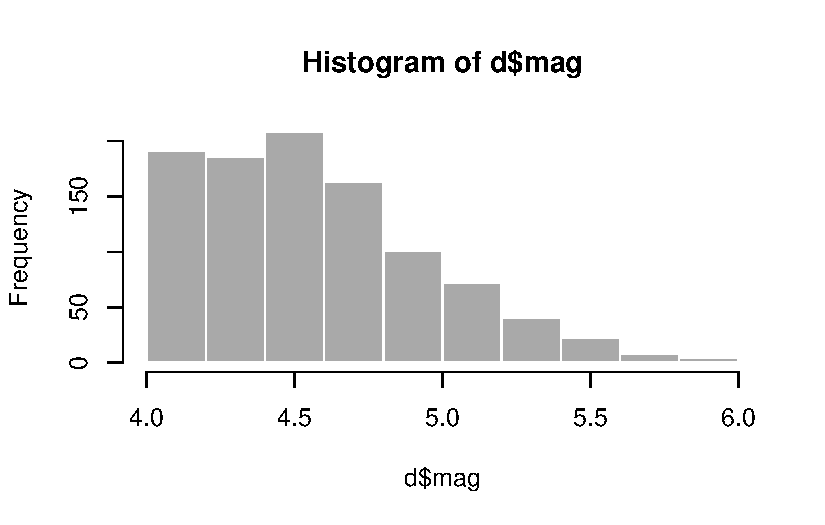
\includegraphics{./shiny_files/figure-pdf/unnamed-chunk-6-1.pdf}

}

\end{figure}

\begin{itemize}
\item
  Code:
  \href{https://github.com/bbest/shiny-intro/tree/master/02_quakes_mag}{02\_quakes\_mag}
\item
  Run from GitHub:

\begin{Shaded}
\begin{Highlighting}[]
\NormalTok{shiny}\SpecialCharTok{::}\FunctionTok{runGitHub}\NormalTok{(}\StringTok{"bbest/shiny{-}intro"}\NormalTok{, }\AttributeTok{subdir=}\StringTok{"02\_quakes\_mag"}\NormalTok{)}
\end{Highlighting}
\end{Shaded}
\item
  Run locally:

\begin{Shaded}
\begin{Highlighting}[]
\NormalTok{shiny}\SpecialCharTok{::}\FunctionTok{runApp}\NormalTok{(}\StringTok{"02\_quakes\_mag"}\NormalTok{)}
\end{Highlighting}
\end{Shaded}
\end{itemize}

\hypertarget{quakes_depth}{%
\subsection{\texorpdfstring{\texttt{03\_quakes\_depth}}{03\_quakes\_depth}}\label{quakes_depth}}

\begin{Shaded}
\begin{Highlighting}[]
\FunctionTok{library}\NormalTok{(tidyverse)}

\NormalTok{input }\OtherTok{\textless{}{-}} \FunctionTok{list}\NormalTok{(}
  \AttributeTok{select\_var =} \StringTok{"depth"}\NormalTok{, }
  \AttributeTok{slider\_mag =} \FunctionTok{c}\NormalTok{(}\DecValTok{4}\NormalTok{, }\DecValTok{5}\NormalTok{), }
  \AttributeTok{slider\_depth =} \FunctionTok{c}\NormalTok{(}\DecValTok{0}\NormalTok{, }\DecValTok{100}\NormalTok{))}

\NormalTok{d }\OtherTok{\textless{}{-}}\NormalTok{ quakes }\SpecialCharTok{\%\textgreater{}\%}
  \FunctionTok{filter}\NormalTok{(}
\NormalTok{    mag   }\SpecialCharTok{\textgreater{}=}\NormalTok{ input}\SpecialCharTok{$}\NormalTok{slider\_mag[}\DecValTok{1}\NormalTok{],}
\NormalTok{    mag   }\SpecialCharTok{\textless{}=}\NormalTok{ input}\SpecialCharTok{$}\NormalTok{slider\_mag[}\DecValTok{2}\NormalTok{],}
\NormalTok{    depth }\SpecialCharTok{\textgreater{}=}\NormalTok{ input}\SpecialCharTok{$}\NormalTok{slider\_depth[}\DecValTok{1}\NormalTok{],}
\NormalTok{    depth }\SpecialCharTok{\textless{}=}\NormalTok{ input}\SpecialCharTok{$}\NormalTok{slider\_depth[}\DecValTok{2}\NormalTok{])}

\FunctionTok{hist}\NormalTok{(d[,input}\SpecialCharTok{$}\NormalTok{select\_var], }\AttributeTok{col =} \StringTok{\textquotesingle{}darkgray\textquotesingle{}}\NormalTok{, }\AttributeTok{border =} \StringTok{\textquotesingle{}white\textquotesingle{}}\NormalTok{)}
\end{Highlighting}
\end{Shaded}

\begin{figure}[H]

{\centering 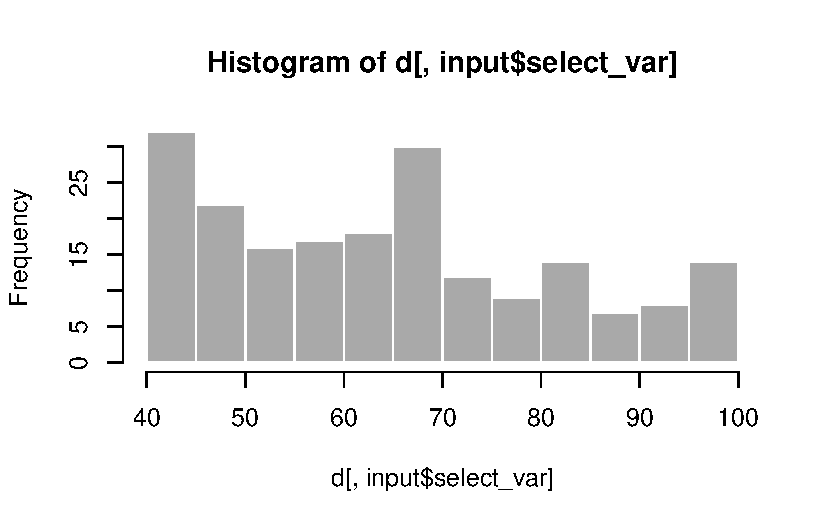
\includegraphics{./shiny_files/figure-pdf/unnamed-chunk-7-1.pdf}

}

\end{figure}

\begin{itemize}
\item
  Code:
  \href{https://github.com/bbest/shiny-intro/tree/master/03_quakes_depth}{03\_quakes\_depth}
\item
  Run from GitHub:

\begin{Shaded}
\begin{Highlighting}[]
\NormalTok{shiny}\SpecialCharTok{::}\FunctionTok{runGitHub}\NormalTok{(}\StringTok{"bbest/shiny{-}intro"}\NormalTok{, }\AttributeTok{subdir=}\StringTok{"03\_quakes\_depth"}\NormalTok{)}
\end{Highlighting}
\end{Shaded}
\item
  Run locally:

\begin{Shaded}
\begin{Highlighting}[]
\NormalTok{shiny}\SpecialCharTok{::}\FunctionTok{runApp}\NormalTok{(}\StringTok{"03\_quakes\_depth"}\NormalTok{)}
\end{Highlighting}
\end{Shaded}
\item
  \href{https://github.com/bbest/shiny-intro/tree/master/04_quakes_map}{shiny-intro/04\_quakes\_map
  at master · bbest/shiny-intro}
\item
  \href{https://github.com/bbest/shiny-intro/tree/master/05_quakes_dashboard}{shiny-intro/05\_quakes\_dashboard
  at master · bbest/shiny-intro}
\item
  \href{http://benbestphd.com/shiny-intro/crosstalk.html}{Fiji
  earthquakes}
\end{itemize}

\hypertarget{quakes_map}{%
\subsection{\texorpdfstring{\texttt{04\_quakes\_map}}{04\_quakes\_map}}\label{quakes_map}}

\begin{itemize}
\tightlist
\item
  \href{http://rstudio.github.io/leaflet/markers.html\#icon-markers}{Leaflet
  for R - Markers}
\end{itemize}

\begin{Shaded}
\begin{Highlighting}[]
\FunctionTok{library}\NormalTok{(leaflet)}
\FunctionTok{library}\NormalTok{(glue)}

\FunctionTok{leaflet}\NormalTok{(}\AttributeTok{data =}\NormalTok{ quakes[}\DecValTok{1}\SpecialCharTok{:}\DecValTok{20}\NormalTok{,]) }\SpecialCharTok{\%\textgreater{}\%} 
  \FunctionTok{addTiles}\NormalTok{() }\SpecialCharTok{\%\textgreater{}\%}
  \FunctionTok{addCircleMarkers}\NormalTok{(}
    \AttributeTok{radius =} \SpecialCharTok{\textasciitilde{}}\NormalTok{mag, }\AttributeTok{color =} \StringTok{"red"}\NormalTok{, }\AttributeTok{stroke =} \ConstantTok{FALSE}\NormalTok{, }\AttributeTok{fillOpacity =} \FloatTok{0.5}\NormalTok{,}
    \AttributeTok{popup =} \SpecialCharTok{\textasciitilde{}}\FunctionTok{glue}\NormalTok{(}\StringTok{"\textless{}b\textgreater{}mag\textless{}/b\textgreater{}: \{mag\}\textless{}br\textgreater{}depth: \{depth\} m"}\NormalTok{), }\AttributeTok{label =} \SpecialCharTok{\textasciitilde{}}\FunctionTok{as.character}\NormalTok{(mag))}
\end{Highlighting}
\end{Shaded}

\begin{itemize}
\item
  Code:
  \href{https://github.com/bbest/shiny-intro/tree/master/04_quakes_map}{04\_quakes\_map}
\item
  Run from GitHub:

\begin{Shaded}
\begin{Highlighting}[]
\NormalTok{shiny}\SpecialCharTok{::}\FunctionTok{runGitHub}\NormalTok{(}\StringTok{"bbest/shiny{-}intro"}\NormalTok{, }\AttributeTok{subdir=}\StringTok{"04\_quakes\_map"}\NormalTok{)}
\end{Highlighting}
\end{Shaded}
\item
  Run locally:

\begin{Shaded}
\begin{Highlighting}[]
\NormalTok{shiny}\SpecialCharTok{::}\FunctionTok{runApp}\NormalTok{(}\StringTok{"04\_quakes\_map"}\NormalTok{)}
\end{Highlighting}
\end{Shaded}
\end{itemize}

\hypertarget{quakes_dashboard}{%
\subsection{\texorpdfstring{\texttt{05\_quakes\_dashboard}}{05\_quakes\_dashboard}}\label{quakes_dashboard}}

Use:

\begin{itemize}
\item
  \href{http://rstudio.github.io/shinydashboard}{shinydashboard}
\item
  \href{https://github.com/tidyverse/ggplot2}{ggplot2}
\item
  \href{https://plot.ly/ggplot2}{plot.ly}
\end{itemize}

\begin{Shaded}
\begin{Highlighting}[]
\FunctionTok{library}\NormalTok{(tidyverse)}
\FunctionTok{library}\NormalTok{(glue)}

\NormalTok{input }\OtherTok{\textless{}{-}} \FunctionTok{list}\NormalTok{(}
  \AttributeTok{select\_var   =} \StringTok{"depth"}\NormalTok{, }
  \AttributeTok{slider\_mag   =} \FunctionTok{c}\NormalTok{(}\DecValTok{4}\NormalTok{, }\DecValTok{5}\NormalTok{), }
  \AttributeTok{slider\_depth =} \FunctionTok{c}\NormalTok{(}\DecValTok{0}\NormalTok{, }\DecValTok{100}\NormalTok{))}

\NormalTok{get\_df }\OtherTok{\textless{}{-}} \ControlFlowTok{function}\NormalTok{()\{}
\NormalTok{  df }\OtherTok{\textless{}{-}}\NormalTok{ quakes }\SpecialCharTok{\%\textgreater{}\%}
    \FunctionTok{filter}\NormalTok{(}
\NormalTok{      mag   }\SpecialCharTok{\textgreater{}=}\NormalTok{ input}\SpecialCharTok{$}\NormalTok{slider\_mag[}\DecValTok{1}\NormalTok{],}
\NormalTok{      mag   }\SpecialCharTok{\textless{}=}\NormalTok{ input}\SpecialCharTok{$}\NormalTok{slider\_mag[}\DecValTok{2}\NormalTok{],}
\NormalTok{      depth }\SpecialCharTok{\textgreater{}=}\NormalTok{ input}\SpecialCharTok{$}\NormalTok{slider\_depth[}\DecValTok{1}\NormalTok{],}
\NormalTok{      depth }\SpecialCharTok{\textless{}=}\NormalTok{ input}\SpecialCharTok{$}\NormalTok{slider\_depth[}\DecValTok{2}\NormalTok{])}
\NormalTok{  df}\SpecialCharTok{$}\NormalTok{var }\OtherTok{\textless{}{-}}\NormalTok{ df[[input}\SpecialCharTok{$}\NormalTok{select\_var]]}
\NormalTok{  df}
\NormalTok{\}}

\NormalTok{df        }\OtherTok{\textless{}{-}} \FunctionTok{get\_df}\NormalTok{()}
\NormalTok{bin\_width }\OtherTok{\textless{}{-}} \FunctionTok{min}\NormalTok{(}\FunctionTok{c}\NormalTok{(}\DecValTok{7}\NormalTok{, }\FunctionTok{length}\NormalTok{(}\FunctionTok{unique}\NormalTok{(df}\SpecialCharTok{$}\NormalTok{var))))}
    
\NormalTok{g }\OtherTok{\textless{}{-}} \FunctionTok{ggplot}\NormalTok{(df, }\FunctionTok{aes}\NormalTok{(var)) }\SpecialCharTok{+} 
  \FunctionTok{geom\_histogram}\NormalTok{(}\AttributeTok{binwidth=}\NormalTok{bin\_width)}

\NormalTok{plotly}\SpecialCharTok{::}\FunctionTok{ggplotly}\NormalTok{(g)}
\end{Highlighting}
\end{Shaded}

\begin{itemize}
\item
  Code:
  \href{https://github.com/bbest/shiny-intro/tree/master/05_quakes_dashboard}{05\_quakes\_dashboard}
\item
  Run from GitHub:

\begin{Shaded}
\begin{Highlighting}[]
\NormalTok{shiny}\SpecialCharTok{::}\FunctionTok{runGitHub}\NormalTok{(}\StringTok{"bbest/shiny{-}intro"}\NormalTok{, }\AttributeTok{subdir=}\StringTok{"05\_quakes\_dashboard"}\NormalTok{)}
\end{Highlighting}
\end{Shaded}
\item
  Run locally:

\begin{Shaded}
\begin{Highlighting}[]
\NormalTok{shiny}\SpecialCharTok{::}\FunctionTok{runApp}\NormalTok{(}\StringTok{"05\_quakes\_dashboard"}\NormalTok{)}
\end{Highlighting}
\end{Shaded}
\item
  View app directly:
  \url{https://bdbest.shinyapps.io/05_quakes_dashboard}

  \begin{figure}

  {\centering 

  \href{https://bdbest.shinyapps.io/05_quakes_dashboard}{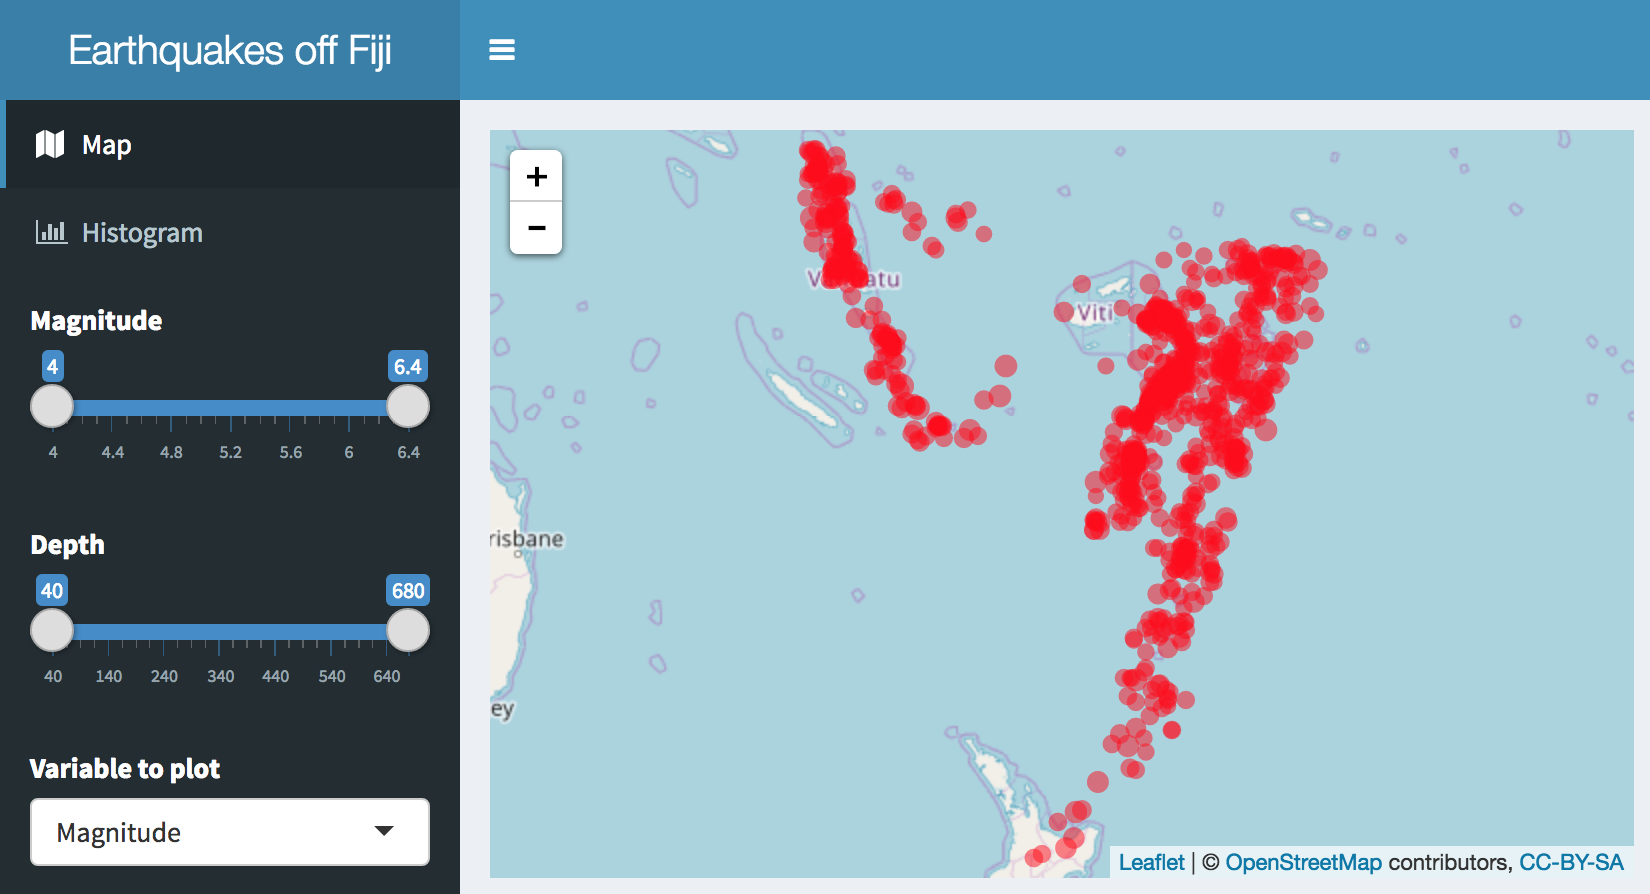
\includegraphics{./figs/shiny/screenshot-05_quakes_dashboard.png}}

  }

  \end{figure}
\end{itemize}

\hypertarget{rmarkdown-using-crosstalk}{%
\section{Rmarkdown using Crosstalk}\label{rmarkdown-using-crosstalk}}

\begin{itemize}
\tightlist
\item
  \url{https://rstudio.github.io/crosstalk}
\end{itemize}

\begin{Shaded}
\begin{Highlighting}[]
\FunctionTok{library}\NormalTok{(crosstalk)}
\FunctionTok{library}\NormalTok{(leaflet)}
\FunctionTok{library}\NormalTok{(DT)}

\CommentTok{\# Wrap data frame in SharedData}
\NormalTok{sd }\OtherTok{\textless{}{-}}\NormalTok{ SharedData}\SpecialCharTok{$}\FunctionTok{new}\NormalTok{(quakes[}\FunctionTok{sample}\NormalTok{(}\FunctionTok{nrow}\NormalTok{(quakes), }\DecValTok{100}\NormalTok{),])}

\CommentTok{\# Create a filter input}
\FunctionTok{filter\_slider}\NormalTok{(}\StringTok{"mag"}\NormalTok{, }\StringTok{"Magnitude"}\NormalTok{, sd, }\AttributeTok{column=}\SpecialCharTok{\textasciitilde{}}\NormalTok{mag, }\AttributeTok{step=}\FloatTok{0.1}\NormalTok{, }\AttributeTok{width=}\DecValTok{250}\NormalTok{)}
\end{Highlighting}
\end{Shaded}

\begin{Shaded}
\begin{Highlighting}[]
\CommentTok{\# Use SharedData like a dataframe with Crosstalk{-}enabled widgets}
\FunctionTok{bscols}\NormalTok{(}
  \FunctionTok{leaflet}\NormalTok{(sd) }\SpecialCharTok{\%\textgreater{}\%} 
    \FunctionTok{addTiles}\NormalTok{() }\SpecialCharTok{\%\textgreater{}\%} 
    \FunctionTok{addMarkers}\NormalTok{(),}
  \FunctionTok{datatable}\NormalTok{(}
\NormalTok{    sd, }\AttributeTok{extensions=}\StringTok{"Scroller"}\NormalTok{, }\AttributeTok{style=}\StringTok{"bootstrap"}\NormalTok{, }\AttributeTok{class=}\StringTok{"compact"}\NormalTok{, }\AttributeTok{width=}\StringTok{"100\%"}\NormalTok{,}
    \AttributeTok{options=}\FunctionTok{list}\NormalTok{(}\AttributeTok{deferRender=}\ConstantTok{TRUE}\NormalTok{, }\AttributeTok{scrollY=}\DecValTok{300}\NormalTok{, }\AttributeTok{scroller=}\ConstantTok{TRUE}\NormalTok{)))}
\end{Highlighting}
\end{Shaded}

\hypertarget{further-resources}{%
\section*{Further Resources}\label{further-resources}}
\addcontentsline{toc}{section}{Further Resources}

\markright{Further Resources}

\begin{itemize}
\tightlist
\item
  \href{https://shiny.rstudio.com/articles/cheatsheet.html}{Shiny
  Cheatsheet}
\item
  \href{https://shiny.rstudio.com/tutorial/}{Shiny Tutorial}
\item
  \href{https://www.rstudio.com/resources/webinars/introduction-to-shiny/}{Introduction
  to Shiny - RStudio}
\end{itemize}

\bookmarksetup{startatroot}

\hypertarget{summary}{%
\chapter{Summary}\label{summary}}

In summary, this book has no content whatsoever.

\begin{Shaded}
\begin{Highlighting}[]
\DecValTok{1} \SpecialCharTok{+} \DecValTok{1}
\end{Highlighting}
\end{Shaded}

\begin{verbatim}
[1] 2
\end{verbatim}

\bookmarksetup{startatroot}

\hypertarget{references}{%
\chapter*{References}\label{references}}
\addcontentsline{toc}{chapter}{References}

\markboth{References}{References}

\hypertarget{refs}{}
\begin{CSLReferences}{1}{0}
\leavevmode\vadjust pre{\hypertarget{ref-knuth84}{}}%
Knuth, Donald E. 1984. {``Literate Programming.''} \emph{Comput. J.} 27
(2): 97--111. \url{https://doi.org/10.1093/comjnl/27.2.97}.

\end{CSLReferences}



\end{document}
